\documentclass[a4paper]{article}
\usepackage[utf8]{inputenc}
\usepackage[spanish, es-tabla, es-noshorthands]{babel}
\usepackage[table,xcdraw]{xcolor}
\usepackage[a4paper, footnotesep = 1cm, width=22cm, top=2.5cm, height=25cm, textwidth=20cm, textheight=25cm]{geometry}
%\geometry{showframe}

\usepackage{tikz}
\usepackage{amsmath}
\usepackage{amsfonts}
\usepackage{amssymb}
\usepackage{float}
\usepackage{graphicx}
\usepackage{caption}
\usepackage{subcaption}
\usepackage{multicol}
\usepackage{multirow}
\usepackage{wrapfig}
\setlength{\doublerulesep}{\arrayrulewidth}
\usepackage{booktabs}

\usepackage{hyperref}
\hypersetup{
    colorlinks=true,
    linkcolor=blue,
    filecolor=magenta,      
    urlcolor=blue,
    citecolor=blue,    
}

\newcommand{\note}[1]{
	\begin{center}
		\huge{ \textcolor{red}{#1} }
	\end{center}
}

\setcounter{topnumber}{2}
\setcounter{bottomnumber}{2}
\setcounter{totalnumber}{4}
\renewcommand{\topfraction}{0.85}
\renewcommand{\bottomfraction}{0.85}
\renewcommand{\textfraction}{0.15}
\renewcommand{\floatpagefraction}{0.8}
\renewcommand{\textfraction}{0.1}
\setlength{\floatsep}{5pt plus 2pt minus 2pt}
\setlength{\textfloatsep}{5pt plus 2pt minus 2pt}
\setlength{\intextsep}{5pt plus 2pt minus 2pt}

\newcommand{\quotes}[1]{``#1''}
\usepackage{array}
\newcolumntype{C}[1]{>{\centering\let\newline\\\arraybackslash\hspace{0pt}}m{#1}}
\usepackage[american]{circuitikz}
\usetikzlibrary{calc}
\usepackage{fancyhdr}
\usepackage{units} 

\graphicspath{{../Ejercicio-1/}{../Ejercicio-2/}{../Ejercicio-3/}{../Ejercicio-4/}}

\pagestyle{fancy}
\fancyhf{}
\lhead{31.99 -  Mecatrónica Aplicada}
\rhead{Lambertucci}
\rfoot{Página \thepage}


\begin{document}

%%%%%%%%%%%%%%%%%%%%%%%%%
%		Caratula		%
%%%%%%%%%%%%%%%%%%%%%%%%%

\begin{titlepage}
\newcommand{\HRule}{\rule{\linewidth}{0.5mm}}
\center
\mbox{\textsc{\LARGE \bfseries {Instituto Tecnológico de Buenos Aires}}}\\[1.5cm]
\textsc{\Large 31.99 -  Mecatrónica Aplicada}\\[0.5cm]


\HRule \\[0.6cm]
{ \Huge \bfseries Trabajo práctico N$^{\circ}$I}\\[0.4cm] 
{\huge One Wheel}\\
\HRule \\[1.5cm]


{\large

\emph{Alumno}\\
\vspace{3px}

\begin{tabular}{lr} 	
\textsc{Lambertucci}, Guido Enrique  & 58009 \\
\end{tabular}

\vspace{20px}

\emph{Profesores}\\

\textsc{Perfumo}, Lucas Alberto\\
\textsc{Basualdo}, Hernán Federico\\




\vspace{3px}
%\textsc{} \\	

\vspace{100px}

\begin{tabular}{ll}

Presentado: & 18/08/21\\

\end{tabular}

}

\vfill

\end{titlepage}


%%%%%%%%%%%%%%%%%%%%%
%		Indice		%
%%%%%%%%%%%%%%%%%%%%%

\tableofcontents
\newpage

%%%%%%%%%%%%%%%%%%%%%
%		Informe		%
%%%%%%%%%%%%%%%%%%%%%


\section{Introducci\'on}

En el siguiente trabajo de ingenier\'ia inversa se eligi\'o como producto el One Wheel.
Es una patineta el\'ectrica usada mayormente con fines recreativos,aunque tambi\'en es utilizada para transporte.
%Describan el proyecto en forma general y sintética (uso, función, finalidad, etc). Campos de aplicación y antecedentes.
\begin{figure}[H]
	\center
	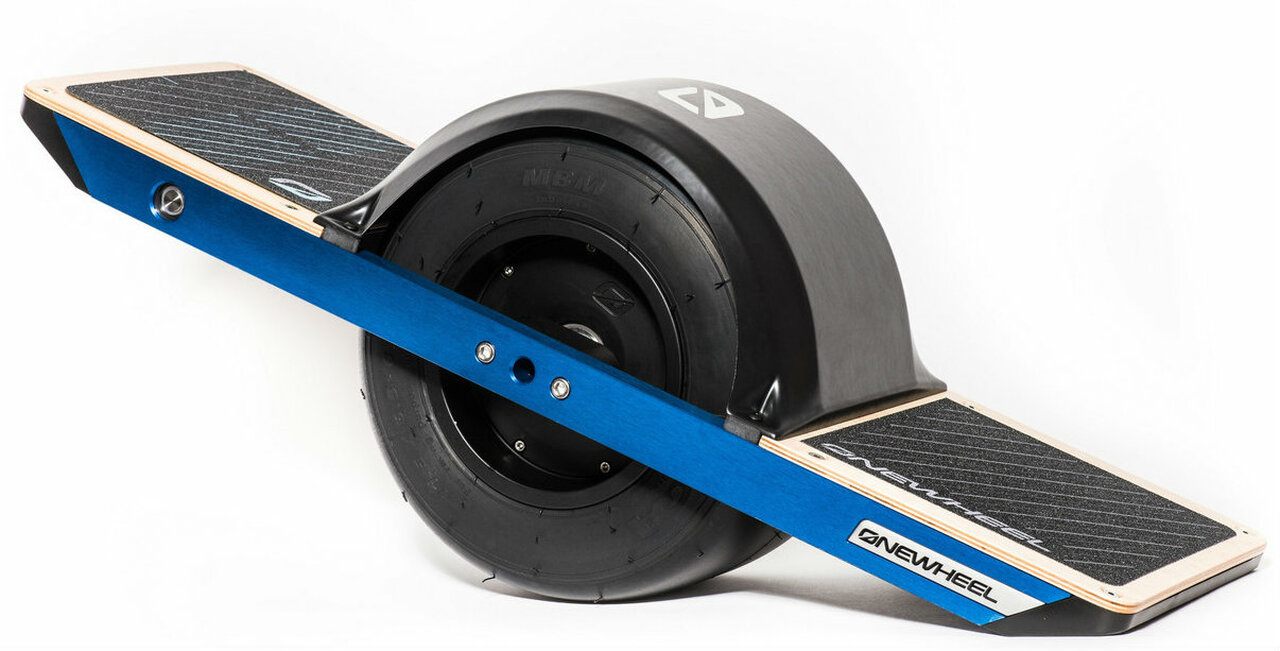
\includegraphics[width=0.6\linewidth, page=1]{Imagenes/onewheel}
	\caption{OneWheel.}
	\label{fig:intro:OneWheel}
\end{figure}
\subsection{Uso}
Para su uso basta con colocar los pies sobre las superficies con lija e impulsarse para poner la patineta en posición horizontal. Esto activar\'a el sistema de balance autom\'atico de la patineta, el cual equilibrar\'a la tabla en posci\'on horizontal. Para acelerar basta con desplazar el peso de uno en la dirección deseada, lo cual indicar\'a a la tabla el cambio que debe hacer.
\subsection{Alternativas}
En el mercado existe otras alternativas similares al OneWheel tales como el monociclo eléctrico.
 \begin{figure}[H]
	\center
	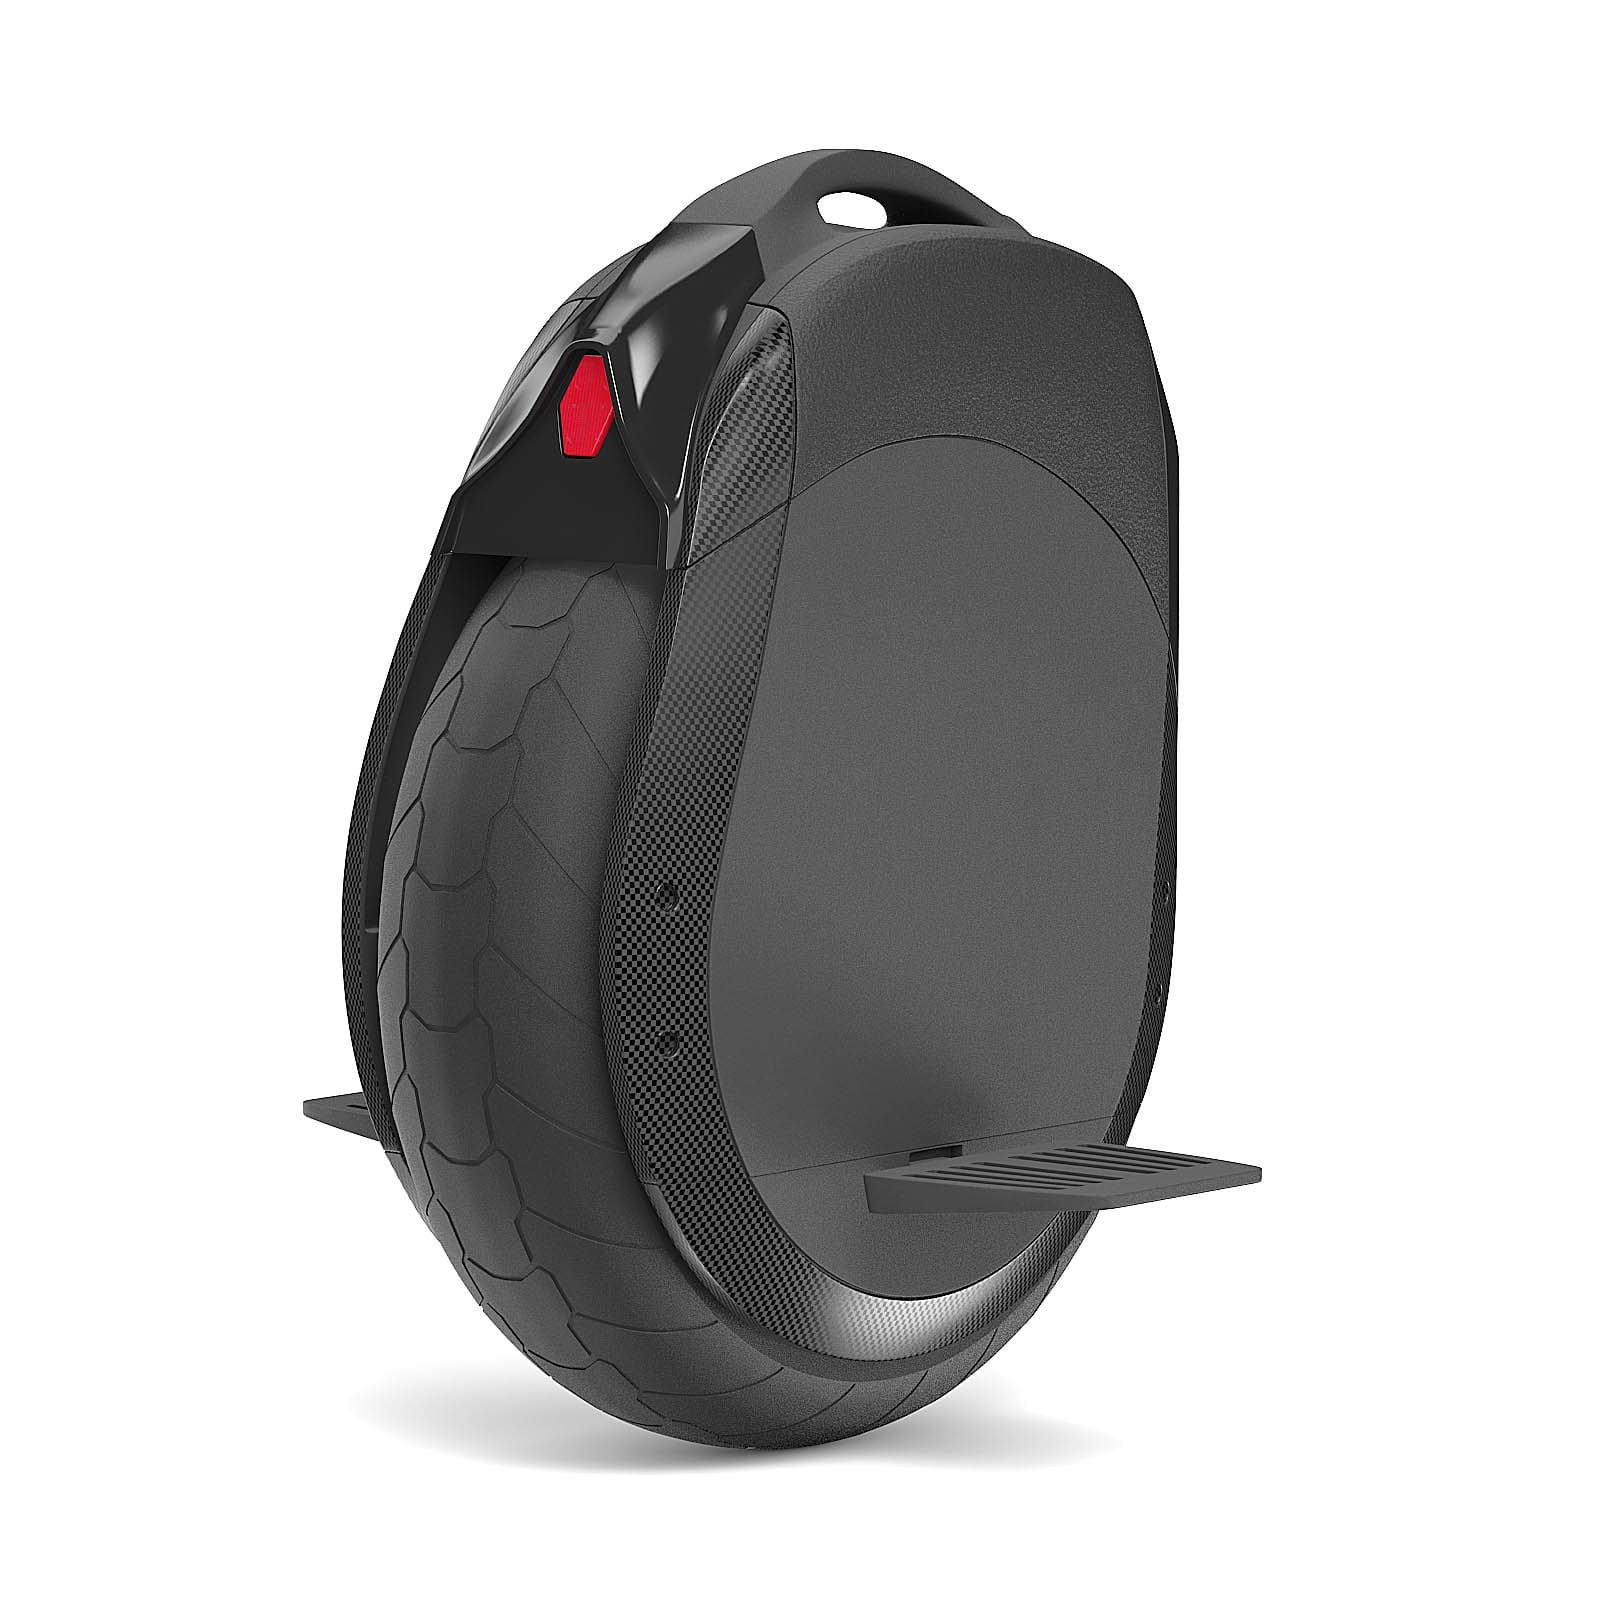
\includegraphics[width=0.4\linewidth, page=1]{Imagenes/antescedentes}
	\caption{Monociclo el\'ectrico.}
	\label{fig:intro:monociclo_electrico}
\end{figure}
Algunas características en las que difieren estas dos alternativas son: la posici\'on en la que uno pone las piernas, la direcci\'on de avance (con los pies ortogonales al movimiento o no)
el tamaño y el perfil de uso.
\section{Esquema f\'isico}
El OneWheel está compuesto por diversas partes dentro de ellas se pueden mencionar los siguientes elementos
 \begin{figure}[H]
	\center
	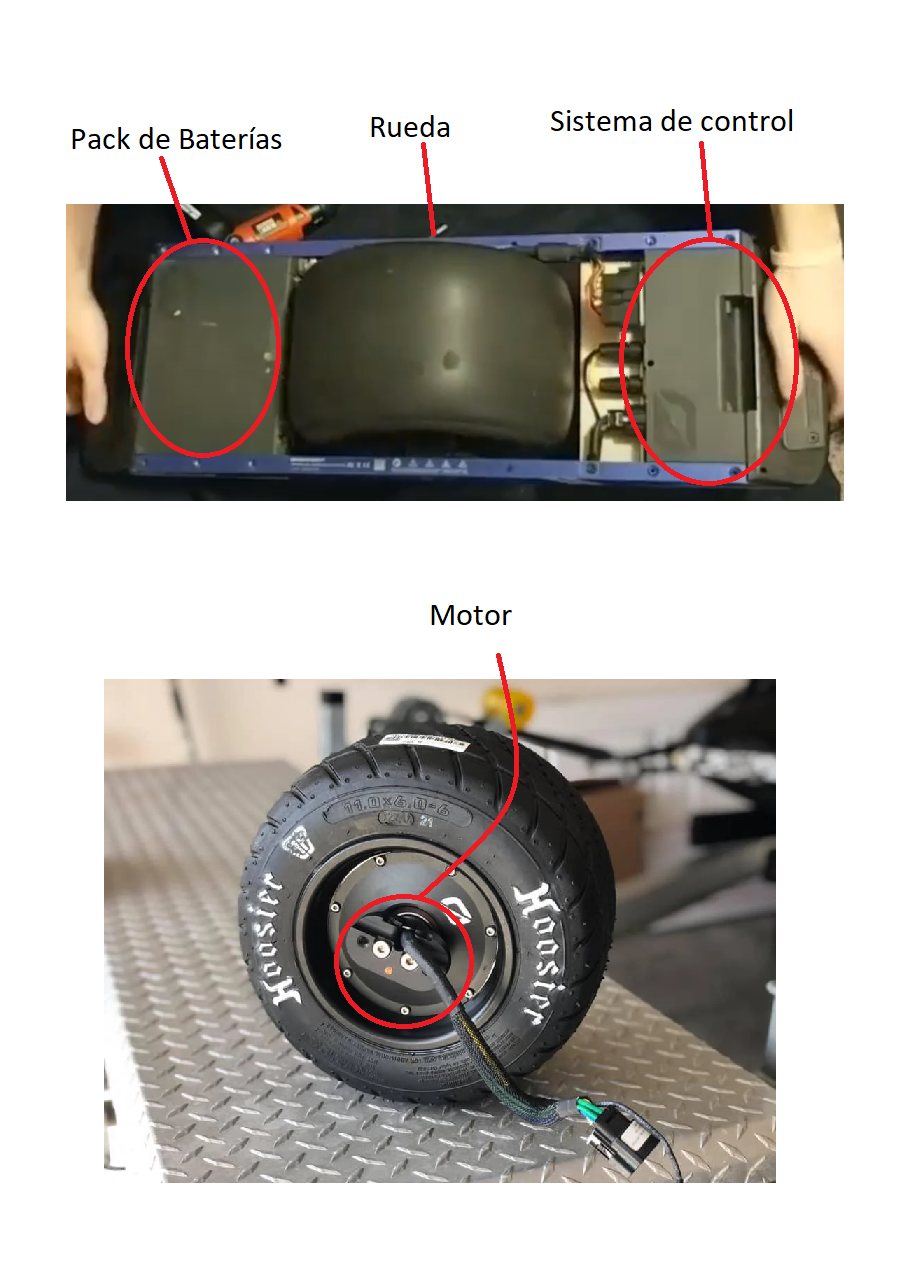
\includegraphics[width=0.4\linewidth, page=1]{Imagenes/Diagrama}
	\caption{Esquema de componentes.}
	\label{fig:Esq_fisico:diagrama}
\end{figure}
Ademas en la unidad de control se distinguen una unidad de medidas inerciales (IMU), algún microcontrolador (MCU) para realizar el control programable, baterías, rueda, una carcasa con antideslizantes. 



%Su función global, funcionamiento y sus partes constitutivas (Descriptivo y sintético); pueden resolver a mano alzada o capturando imágenes representativas.

\section{Esquema de control}
\subsection{Variable de medici\'on}
Las variables de medición son el ángulo respecto de la normal a la tierra. Ya que en el sistema de control de balance automático tiene como finalidad mantener el ángulo ortogonal al piso, el control de velocidad es realizado por otro sistema.
  
\subsection{Sensores}
Los sensores utilizados en el sistema de balance automático del OneWheel son:
\begin{itemize}
\item Aceler\'ometro
\item Magnetómetro
\item Giróscopo
\end{itemize}
\subsubsection{Aceler\'ometro}
\subsubsection{Magnetómetro}
\subsubsection{Giróscopo}
\subsubsection{Sensor fusion}
La t\'ecnica de \textit{sensor fusion} consiste en combinar las mediciones de por lo menos 2 fuentes de informaci\'on en una manera que genere un \textbf{mejor entendimiento} del sistema estudiado. Donde por mejor entendimiento se interpreta como mas consistente, mas preciso, mas confiable.

\subsection{Actuadores}
\subsubsection{Motores}
\subsection{Lazo de control propuesto}
\subsubsection{Lazo de control}
\begin{figure}[H]
	\center
	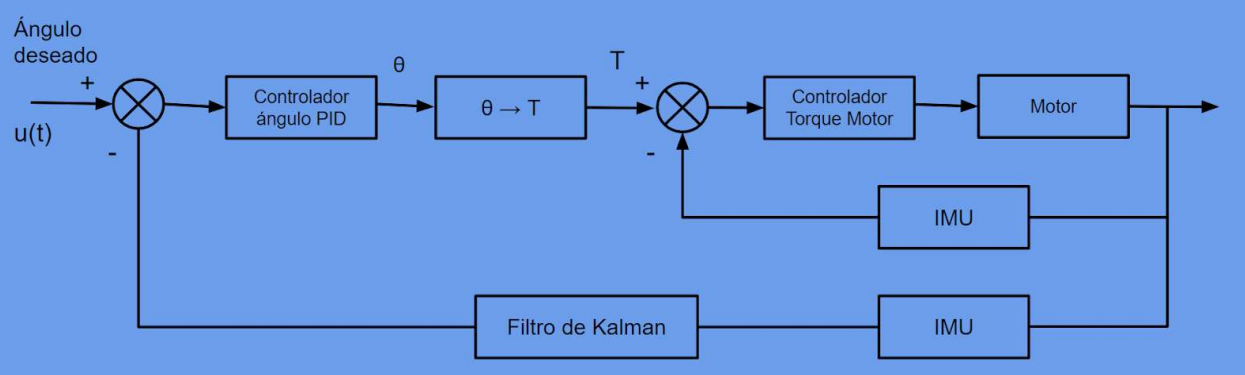
\includegraphics[width=1\linewidth, page=1]{Imagenes/lazo_de_control}
	\caption{Lazo de control.}
	\label{fig:control:lazo}
\end{figure}

\subsubsection{Motores FOC}
\subsubsection{Kalman Filter}


%Esquema preeliminar de control (lógica gral.) Sensores y actuadores que intervienen (no deben seleccionar o definir los componentes; solo dar una idea de qué se podría utilizar en cada caso o cual es el parámetro o variable que deberían medir).

\end{document}
